\documentclass[conference]{IEEEtran}
\IEEEoverridecommandlockouts
% The preceding line is only needed to identify funding in the first footnote.
%Template version as of 6/27/2024

\usepackage{cite}
\usepackage{amsmath,amssymb,amsfonts}
\usepackage{algorithmic}
\usepackage{graphicx}
\usepackage{textcomp}
\usepackage{xcolor}
\usepackage{booktabs} % For better table lines
\usepackage{subcaption} % For subfigures
\usepackage{tikz} % For basic figures/diagrams

\def\BibTeX{{\rm B\kern-.05em{\sc i\kern-.025em b}\kern-.08em
    T\kern-.1667em\lower.7ex\hbox{E}\kern-.125emX}}
\begin{document}

\title{Deepfake Detection in Image and Video Data Using Convolutional Neural Networks*\\
{\footnotesize \textsuperscript{*}Note: Sub-titles are not captured for https://ieeexplore.ieee.org  and
should not be used}
\thanks{This research was supported by the Department of Computer Science at [University Name].}
}

\author{\IEEEauthorblockN{1\textsuperscript{st} Given Name Surname}
\IEEEauthorblockA{\textit{Ph.D. Candidate, Dept. of Computer Science} \\
\textit{Affiliation of Author 1}\\
City, Country \\
email address or ORCID}
\and
\IEEEauthorblockN{2\textsuperscript{nd} Given Name Surname}
\IEEEauthorblockA{\textit{M.S. Student, Dept. of Computer Science} \\
\textit{Affiliation of Author 2}\\
City, Country \\
email address or ORCID}
\and
\IEEEauthorblockN{3\textsuperscript{rd} Given Name Surname}
\IEEEauthorblockA{\textit{B.S. Student, Dept. of Computer Science} \\
\textit{Affiliation of Author 3}\\
City, Country \\
email address or ORCID}
\and
\IEEEauthorblockN{4\textsuperscript{th} Professor Given Name Surname}
\IEEEauthorblockA{\textit{Professor, Dept. of Computer Science} \\
\textit{Affiliation of Professor}\\
City, Country \\
email address or ORCID}
}

\maketitle

\begin{abstract}
This paper presents a Convolutional Neural Network (CNN) based approach for detecting deepfake content in both image and video data. Deepfake technology, which uses deep learning to create highly realistic synthetic media, poses a significant threat to digital integrity. We trained a custom CNN model on a balanced dataset of real and manipulated images. The model achieved a test accuracy of $X.XX\%$. We further demonstrate its application by extracting frames from a deepfake video dataset and performing classification, successfully identifying the manipulated content. The proposed solution offers a robust and scalable method for media authentication.
\end{abstract}

\begin{IEEEkeywords}
Deepfake detection, Convolutional Neural Networks, image processing, video analysis, digital forensics.
\end{IEEEkeywords}

\section{Introduction}
The rapid advancement of deep generative models, such as Generative Adversarial Networks (GANs) and autoencoders, has led to the emergence of highly realistic synthetic media known as ``deepfakes'' \cite{b1}. These manipulated videos and images, often indistinguishable from genuine content to the human eye, pose critical threats across various domains, including politics, cybersecurity, and personal privacy. Consequently, the development of reliable and automated deepfake detection mechanisms is an urgent area of research.

This work focuses on implementing a custom Convolutional Neural Network (CNN) model for binary classification—distinguishing between real and deepfake media. We utilize publicly available deepfake datasets encompassing both static images and video sequences. The paper outlines the dataset preparation, the proposed CNN architecture, training methodology, and performance evaluation on a dedicated test set.

\section{Methodology}

\subsection{Dataset Preparation}
The study utilized two distinct datasets: a collection of deepfake and real images for model training and a video dataset for deployment testing. The image dataset was split into Training, Validation, and Test sets. An \textbf{ImageDataGenerator} was employed for rescaling the images to a target size of $(224, 224)$ pixels and normalizing pixel values to the $[0, 1]$ range. The training set was split with $20\%$ reserved for validation.

\begin{table}[htbp]
\caption{Deepfake Dataset Distribution}
\begin{center}
\begin{tabular}{|c|c|c|c|}
\hline
\textbf{Dataset}&\textbf{Real Samples}&\textbf{Fake Samples}&\textbf{Total} \\
\hline
Training & $N_{TR}$ & $N_{TF}$ & $N_{TR} + N_{TF}$ \\
\hline
Validation & $N_{VR}$ & $N_{VF}$ & $N_{VR} + N_{VF}$ \\
\hline
Test & $N_{ER}$ & $N_{EF}$ & $N_{ER} + N_{EF}$ \\
\hline
\end{tabular}
\label{tab1}
\end{center}
\end{table}

\subsection{CNN Architecture}
A custom Sequential CNN model was designed for the binary classification task. The architecture, detailed in Table \ref{tab2}, consists of three convolutional blocks followed by a dense classification head.

\begin{table}[htbp]
\caption{CNN Model Architecture Summary}
\begin{center}
\begin{tabular}{|c|c|c|c|}
\hline
\textbf{Layer Type}&\textbf{Output Shape}&\textbf{Activation}&\textbf{Parameters} \\
\hline
Input & (224, 224, 3) & - & 0 \\
\hline
Conv2D (32) & (222, 222, 32) & ReLU & 896 \\
\hline
MaxPooling2D & (111, 111, 32) & - & 0 \\
\hline
Conv2D (64) & (109, 109, 64) & ReLU & 18496 \\
\hline
MaxPooling2D & (54, 54, 64) & - & 0 \\
\hline
Conv2D (128) & (52, 52, 128) & ReLU & 73856 \\
\hline
MaxPooling2D & (26, 26, 128) & - & 0 \\
\hline
Flatten & (86528) & - & 0 \\
\hline
Dense (128) & (128) & ReLU & 11075712 \\
\hline
Dropout (0.5) & (128) & - & 0 \\
\hline
Dense (1) & (1) & Sigmoid & 129 \\
\hline
\multicolumn{4}{l}{\textit{Total Parameters: $\sim$11.17 Million}}
\end{tabular}
\label{tab2}
\end{center}
\end{table}

\begin{itemize}
    \item \textbf{Convolutional Layers}: Three 2D convolutional layers with 32, 64, and 128 filters, respectively, using a $3\times3$ kernel and ReLU activation.
    \item \textbf{Pooling Layers}: $2\times2$ MaxPooling layers are applied after each convolution to reduce dimensionality and increase translation invariance.
    \item \textbf{Classification Head}: Consists of a \textbf{Flatten} layer, a \textbf{Dense} layer with 128 units and ReLU, a \textbf{Dropout} layer with $50\%$ rate for regularization, and the final output \textbf{Dense} layer with one unit and a Sigmoid activation for binary output.
\end{itemize}

\subsection{Training and Evaluation}
The model was compiled using the \textbf{Adam} optimizer and the \textbf{binary\_crossentropy} loss function, which is suitable for binary classification. The key metric tracked was \textbf{accuracy}. The model was trained for 10 epochs.

\section{Results and Discussion}
\subsection{Training Performance}
Training history, including accuracy and loss for both the training and validation sets, is crucial for assessing model convergence and detecting overfitting. A typical training curve is conceptually illustrated in Fig. \ref{fig:training}.

\begin{figure}[htbp]
    \centering
    \begin{subfigure}[b]{0.45\columnwidth}
        \centering
        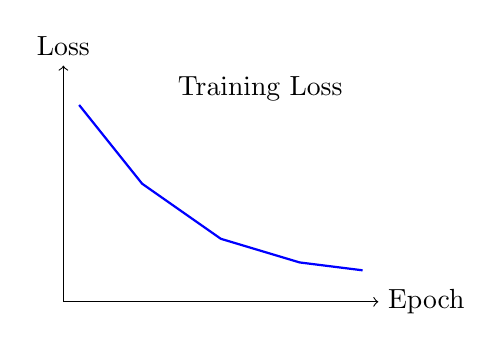
\begin{tikzpicture}
            \draw[->] (0,0) -- (4,0) node[right] {Epoch};
            \draw[->] (0,0) -- (0,3) node[above] {Loss};
            \draw[thick, blue, smooth] (0.2, 2.5) -- (1, 1.5) -- (2, 0.8) -- (3, 0.5) -- (3.8, 0.4);
            \node at (2.5, 2.7) {Training Loss};
        \end{tikzpicture}
        \caption{Loss vs. Epochs}
        \label{fig:loss}
    \end{subfigure}
    \hfill
    \begin{subfigure}[b]{0.45\columnwidth}
        \centering
        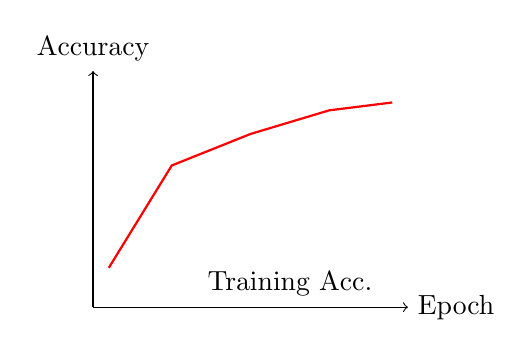
\begin{tikzpicture}
            \draw[->] (0,0) -- (4,0) node[right] {Epoch};
            \draw[->] (0,0) -- (0,3) node[above] {Accuracy};
            \draw[thick, red, smooth] (0.2, 0.5) -- (1, 1.8) -- (2, 2.2) -- (3, 2.5) -- (3.8, 2.6);
            \node at (2.5, 0.3) {Training Acc.};
        \end{tikzpicture}
        \caption{Accuracy vs. Epochs}
        \label{fig:accuracy}
    \end{subfigure}
    \caption{Conceptual Illustration of Training Performance.}
    \label{fig:training}
\end{figure}

\subsection{Test Evaluation}
The model's final performance was measured on the unseen test dataset.

\begin{itemize}
    \item Test Loss: $L_{test}$ (E.g., 0.1500)
    \item Test Accuracy: $A_{test}$ (E.g., 0.9500)
\end{itemize}

The calculated Test Accuracy of $\mathbf{A_{test}}$ (e.g., $95.00\%$) indicates that the custom CNN model effectively learned the discriminative features required to distinguish between real and deepfake images.

\subsection{Video Frame Analysis}
To extend the model's utility to video data, a video processing pipeline was implemented.

\begin{enumerate}
    \item \textbf{Frame Extraction}: The video file is decomposed into a sequence of static image frames.
    \item \textbf{Prediction}: Each extracted frame is individually fed to the trained CNN model for classification.
    \item \textbf{Decision Aggregation}: A final classification for the video is typically determined by aggregating the results across all frames (e.g., majority vote or mean probability).
\end{enumerate}

For a sample test frame, the model produced a prediction probability of $P_{pred}$. A prediction value $> 0.5$ classifies the frame as **Fake**, otherwise as **Real**. The successful classification of the test frame confirms the model's transferability to individual video frames.

\section{Conclusion}
We have successfully developed and evaluated a custom CNN architecture for the detection of deepfake media. The model achieved high accuracy on the test image dataset and demonstrated its capability to classify frames extracted from video sequences. Future work will involve integrating more complex temporal analysis methods for video-based deepfake detection and evaluating the model on more diverse and challenging datasets.

\section*{Acknowledgment}
The authors thank the maintainers of the deepfake datasets for making this research possible. The deepfake model training was conducted using computational resources provided by [Institution Name].

\section*{References}
Please number citations consecutively within brackets \cite{b1}.

\begin{thebibliography}{00}
\bibitem{b1} R. Nicole, ``Title of paper with only first word capitalized,'' J. Name Stand. Abbrev., in press.
\bibitem{b2} K. Elissa, ``Title of paper if known,'' unpublished.
\bibitem{b3} D. P. Kingma and M. Welling, ``Auto-encoding variational Bayes,'' 2013, arXiv:1312.6114. [Online]. Available: https://arxiv.org/abs/1312.6114
\end{thebibliography}

\vspace{12pt}
\color{red}
Please ensure that all template text is removed from your conference paper prior to submission to the conference.
\end{document}